\documentclass{article}
\usepackage{graphicx}
\usepackage{wrapfig}
\usepackage{float}
\usepackage[utf8]{inputenc}
\usepackage[left=2.5cm, right=2.5cm, top=1.25cm, bottom=1.25cm]{geometry}
%\usepackage[colorlinks]{hyperref}
\usepackage[
backend=biber,
style=numeric,
sorting=ynt,
alldates=iso
]{biblatex}
\addbibresource{./assignment2.bib}
\title{Final Report}
\author{Soham Sarfare - 45812748 \and Sukhmani Arora - 45574715 \and Tarun Tirupati - 45532729 \and Ali Saeed - 45853762}
%	\institute{Macquarie University, Sydney NSW 2113, Australia}
	\begin{document}
\maketitle

\tableofcontents

\pagebreak
\begin{abstract}

A research paper in the domain of face detection which has already been published, is replicated and the results have been reproduced, which might prove the appropriateness of the original work by authors, by achieving similar results. Multi-task and extra-supervised learning are utilized in performing a process of face localization with respect to each pixel in the image. This process is a part of a powerful single stage face detector which is termed as RetinaFace. The test dataset has been constructed in which each image from the Wider Face dataset has been annotated manually by recognizing the five facial positions. Pixel-wise shape prediction of these images in the dataset is done using a self-supervised algorithm/code. Further, the difference between the shape of pixels that are manually annotated and the existing data of images with actual pixel shape is observed.
\end{abstract}
\section{Source Paper Description}

The research paper that we are trying to replicate is going to be simple and will involve the stepwise reproducibility. The code and data of this research paper is handled in a manageable way which will include the management of data, explanation of implementation in each step. All the resources that are required for replication and reproduction of results will be mentioned clearly.
The research paper which is replicated is a face localization: RetinaFace research which deals with accurate face detection and efficient localization of a face in an image. Usually it has been seen that a single model cannot accommodate the training of multiple datasets and multiple models are required, but in case of RetinaFace, a single model can be used to train on different datasets containing images, which is an advantage as it is time-saving and localization of facial landmarks can be done in a flexible and simple manner.
\subsection{Evaluation Framework}

In the original work, the dataset contains 32,203 images and 393,703 bounding boxes which are created by annotating the five facial landmarks (eyes centre, nose tip and mouth corners). All these images are quite different from each other in scale, position, illumination, etc. The dataset is divided into training, validation, and test subsets, (40\%,10\%,50\%) respectively. To get bigger sizes of training faces, the images are randomly cropped in a square shape and then resized to 640x640. SGD optimizer was used to train the RetinaFace and four GPUs were required. 

Box voting which uses a certain IoU threshold, flip, multi scale strategies were used to test the Wider Face dataset and perform evaluation. The evaluation is done using the metrics such as average precision (AP) and mean AP (mAP) with different value of IoU to achieve accurate face detectors. The RetinaFace was compared with different algorithms which are used in face detection such as, multi-stage cascade CNN, two-stage CNN, CMS-RCNN, HR, MSCNN, Pyramid Box, ISRN and many more. RetinaFace outperforms other algorithms in case of average precision (AP) evaluation metric and gets the applauding AP in every subset of validation and test sets.

Other evaluation metrics such as normalized mean errors, cumulative error distribution can be used to evaluate the accuracy of five facial landmark. ArcFace verification accuracy is used to evaluate face recognition accuracy. Precision recall curves on the validation and test subsets of WiderFace are generated to interpret and compare the RetinaFace with different algorithms/models in which RetinaFace outstands others.

RetinaFace produces qualitative results and can detect numerous faces (upto 900 out of 1151) in a single image with accurate bounding boxes and efficient prediction of five facial landmarks in each face. The resolution, position, scale, illumination, pose of each face can be detected precisely. Techniques like dense regression can be used to overcome the failure in localization of dense face.
\subsection{Justification}	

The quality of the research paper is justified by looking at the number of citations it has, the core rankings, google scholar discipline ranking. Our research paper, the RetinaFace was published in the IEEE Conference on Computer Vision and Pattern Recognition (May 2019) which has an A1 rating given  by Qualis\footnote{ \url{ http://www.conferenceranks.com/#data} }  and CORE rating of A*\footnote{\url{http://portal.core.edu.au/conf-ranks/604/}}. According to Google Scholar, this research paper has 107 citations\footnote{\url{https://scholar.google.com/scholar?hl=en&as_sdt=0\%2C5&q=RetinaFace\%3A+Single-stage+Dense+Face+Localisation+in+the+Wild+citations&btnG=}}. A Github repository which contains all the codes, datasets, and other resources which were used in building this research paper is available\footnote{\url{https://github.com/deepinsight/insightface/tree/master/RetinaFace}}.

\section{Original Dataset - WiderFace}

The WIDER FACE dataset is currently the largest face detection dataset, of which images selected are the publicly available .They have  choosen 32,203 images and label 393,703 faces with a high degree of variability in scale, pose and occlusion.Images are collected in  following ways. 
\begin{itemize}
\item Event categories were defined and chosen following the Large Scale Ontology for Multimedia
\item Images are retrieved using search engines like Google and Bing. For each category, 1000-3000 images were collected.
\end{itemize}

The data were cleaned by manually examining all the images and filtering out images without human face. Then, similar images in each event category were removed to ensure large diversity in face appearance. A total of 32, 203 images are eventually included in the WIDER FACE dataset.
The WIDER FACE dataset is organized based on 61 event classes. For each event class, data is  randomly selected into 40\%/10\%/50\% data as training, validation and testing sets. Then based on the detection rate of EdgeBox, three levels of difficulty (i.e. Easy, Medium and Hard) are defined by incrementally incorporating hard samples
Research paper defines  five levels of face image quality and annotate by  five facial landmarks (i.e. eye centres, nose tip and mouth corners) on faces that can be annotated from the WIDER FACE training and validation subset. In total, they have annotated 84.6k faces on the training set and 18.5k faces on the validation set. The download size of the original data is 3.42GB and the split in the data is given below:
\begin{center}
\begin{tabular}{|c|c|}
	\hline
Split & Examples \\
\hline
test & 16097 \\
train & 12880\\
validation & 3226\\
\hline
\end{tabular}
\end{center}
\section{Replication of Original Work}
The authors of RetinaFace have developed their work into a full fledged python library ‘Insight face’. The source code to this library can be found at the respective github repository\footnote{\url{https://github.com/deepinsight/insightface}}. In this repository, the original code used for the RetinaFace paper can be found under the RetinaFace subfolder. 
\subsection{Setup}
The repository comes with a well laid out readme file which details steps to recreate the outputs obtained by the authors. The repository is cloned on a Linux based machine. In this case, we have cloned the repository in google drive and used Colab to execute the code within. As Colab uses a Linux backend, this method offered the best compromise between speed and feasibility as none of us had access to a system with sufficient VRAM to execute the code. 

The dataset to be tested is the WIDERFACE dataset which is available at the WiderFace Challenge website\footnote{\url{http://shuoyang1213.me/WIDERFACE/index.html}}. WIDERFACE has 3 classes, Train,Val and Test. All three datasets are uploaded to the cloned repository and organized according to the instructions provided in the readme file. The data folder under the repository has the hierarchy:
\begin{verbatim}
data/retinaface/
    train/
        images/
        label.txt
    val/
        images/
        label.txt
    test/
        images/
        label.txt
\end{verbatim} 

With the original data in place, python dependencies need to be installed. The packages needed for this project which are not pre-installed on Colab are, mxnet, opencv, easydict, Cython. These are installed using the command: 
\begin{verbatim}
pip install mxnet-cu101 opencv-python easydict Cython
\end{verbatim}

On successful installation of the dependencies, the \texttt{make} command is executed to setup the environment.

Finally one of the pretrained models provided by the authors has to be downloaded and stored in the models folder. The model used in this testing is the \texttt{RetinaFace-50} which uses \texttt{ResNet50} as its backbone and can be downloaded from the dropbox link provided by the authors\footnote{\url{https://www.dropbox.com/s/53ftnlarhyrpkg2/retinaface-R50.zip?dl=0}}.

\subsection{Testing}
Once the above steps are complete, we can execute the \texttt{test\_widerface.py} file using the command below to test the RetinaFace-50 model on the WiderFace dataset. 
\begin{verbatim}python test_widerface.py --prefix `./model/R50' --mode=1\end{verbatim} 
\begin{wrapfigure}{r}{0.6\linewidth}
	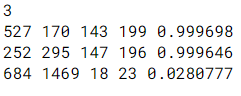
\includegraphics{wout1.png}
	\caption{example of output file}
\end{wrapfigure}  
The output of this process is in form of .txt files, each file corresponding to an image in the dataset. The output file of an image contains the number of faces the model has identified in the image along with the top left (x,y) coordinates, breadth and length of the bounding box made for each face. These outputs are stored under the \texttt{wout} folder.

\subsection{Evaluation}
The labels produced above can be evaluated by the evaluation tools provided on the WiderFace website. These tools are a bunch of MATLAB executable .m files with instructions on how to obtain the outputs. The tools also contain the true labels of the images which are compared to the predicted labels produced by RetinaFace-50 model. Output of these eval tools is in form of Precision-Recall curves per image as shown below. 

\begin{figure}[H]
%	\begin{center}
		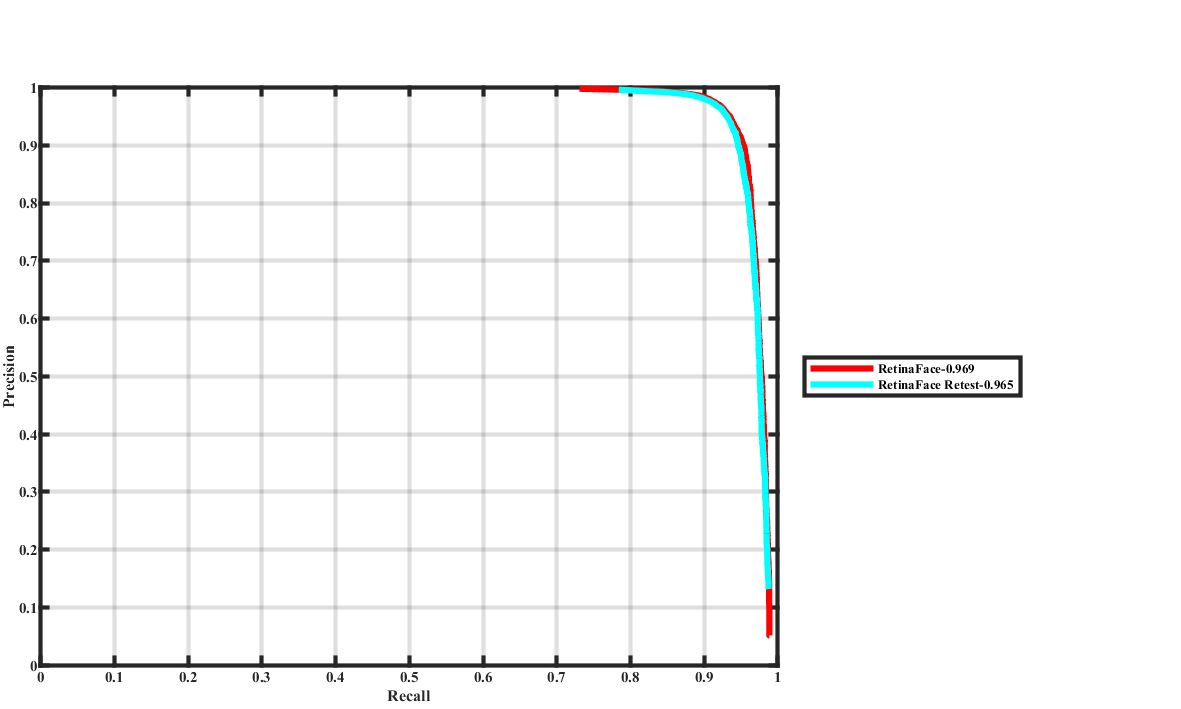
\includegraphics[height=7cm]{wider_pr_cruve_int_easy_val.png}
				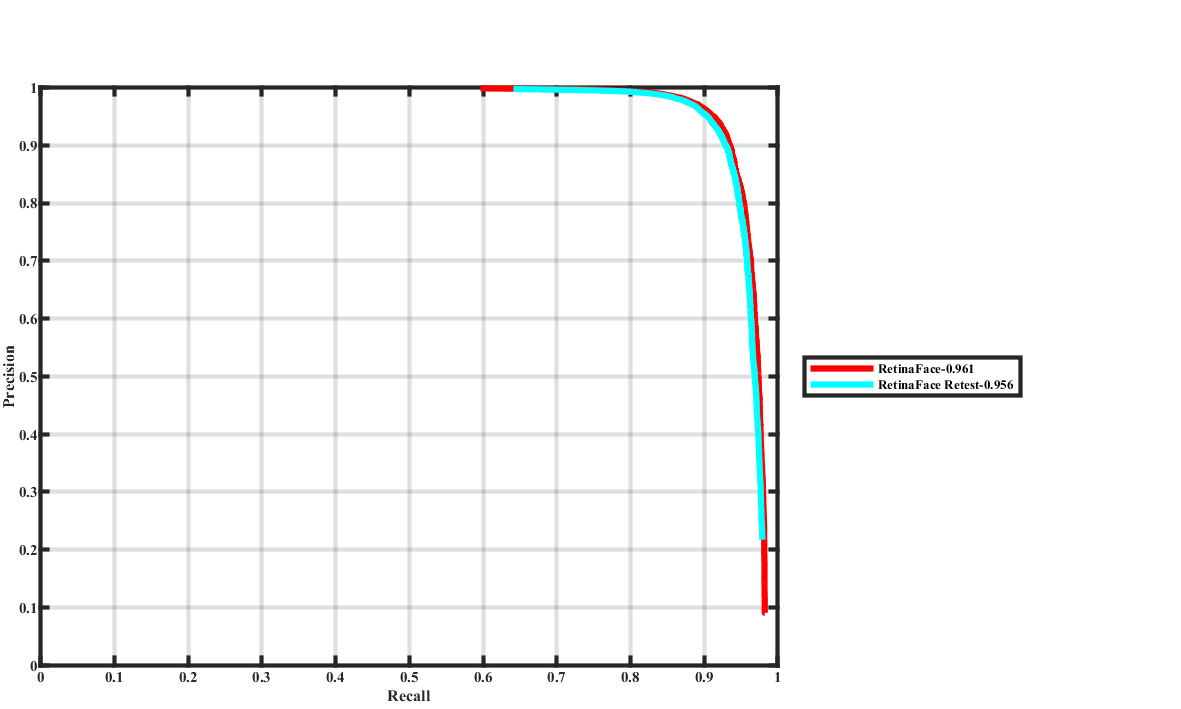
\includegraphics[height=7cm]{wider_pr_cruve_int_medium_val.png}
						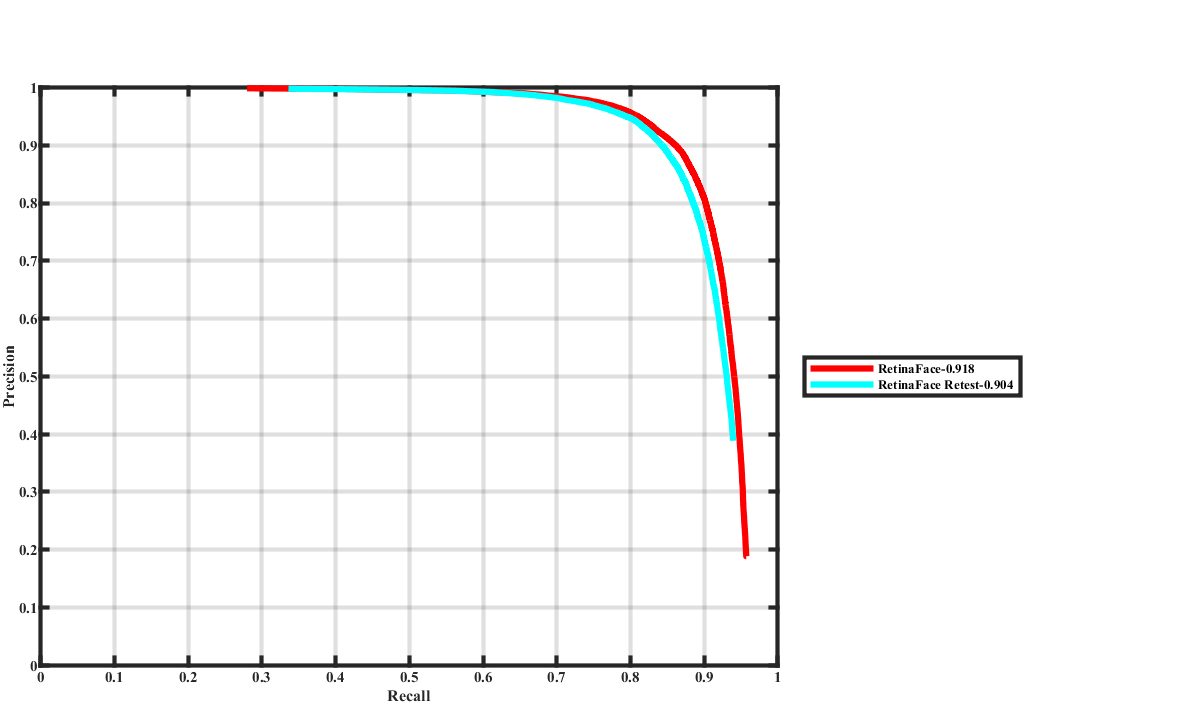
\includegraphics[height=7cm]{wider_pr_cruve_int_hard_val.png}
		\caption{Easy Medium and Hard Validation Sets}
%	\end{center}
\end{figure}

It is evident from the MAP values present in the legend of the graphs above that the retested model performs comparably to the original work of the authors with the values begin within $(1/100)^{ths}$ of one another.
\section{New Dataset}

Our aim is to collect new data that is similar to the original dataset in order to obtain equivalent results as produced in the paper. Hence, we have chosen the process of scraping images using google search engine and the process of web scraping images from few websites.

High resolution images are selected as the initially we have faced complications while running the dataset through the code as the code was unable to identify and locate human facial landmarks due the low image quality. This issue has been rectified by selecting the images that have high resolution and pixel density for the code to run efficiently. 

The new dataset in arranged in such a way that the image data has a high degree of variability in scale, pose, expression, occlusion and illumination which similar to the original dataset .After putting together the dataset of 100 images  our next step was to identify faces that can be annotated in accordance to the outlines specified for the WiderFace dataset. Primarily, the bounding box for these faces had to contain the forehead, cheeks and chin in a tight fit. 

We have manually annotated 100 images by drawing a bounding box coordinates using Microsoft paint application. The annotations have been written into text file in the form of top left (x,y) bounding box coordinates, breadth and length of bounding box The new dataset is then run through the code and evaluation results are observed and documented to check for similarity with original data results.
\begin{figure}[H]
	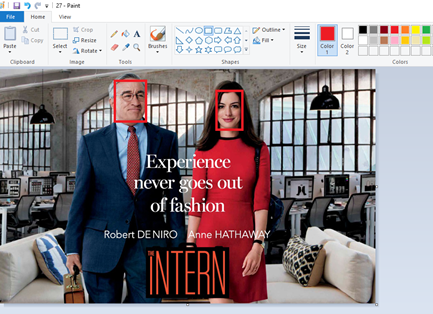
\includegraphics[width=0.5\linewidth]{Picture1.png}
	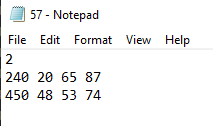
\includegraphics[width=0.5\linewidth]{Picture2.png}
	\caption{Example of New Data Annotation}
\end{figure}

The first two columns define the (x,y) coordinates of the bounding box followed by breadth in the third column and length in the final column.First row indicates the first face in the image starting from left and second row indicated the second human face in the image
\section{Testing on New Data}
\begin{figure}[H]
	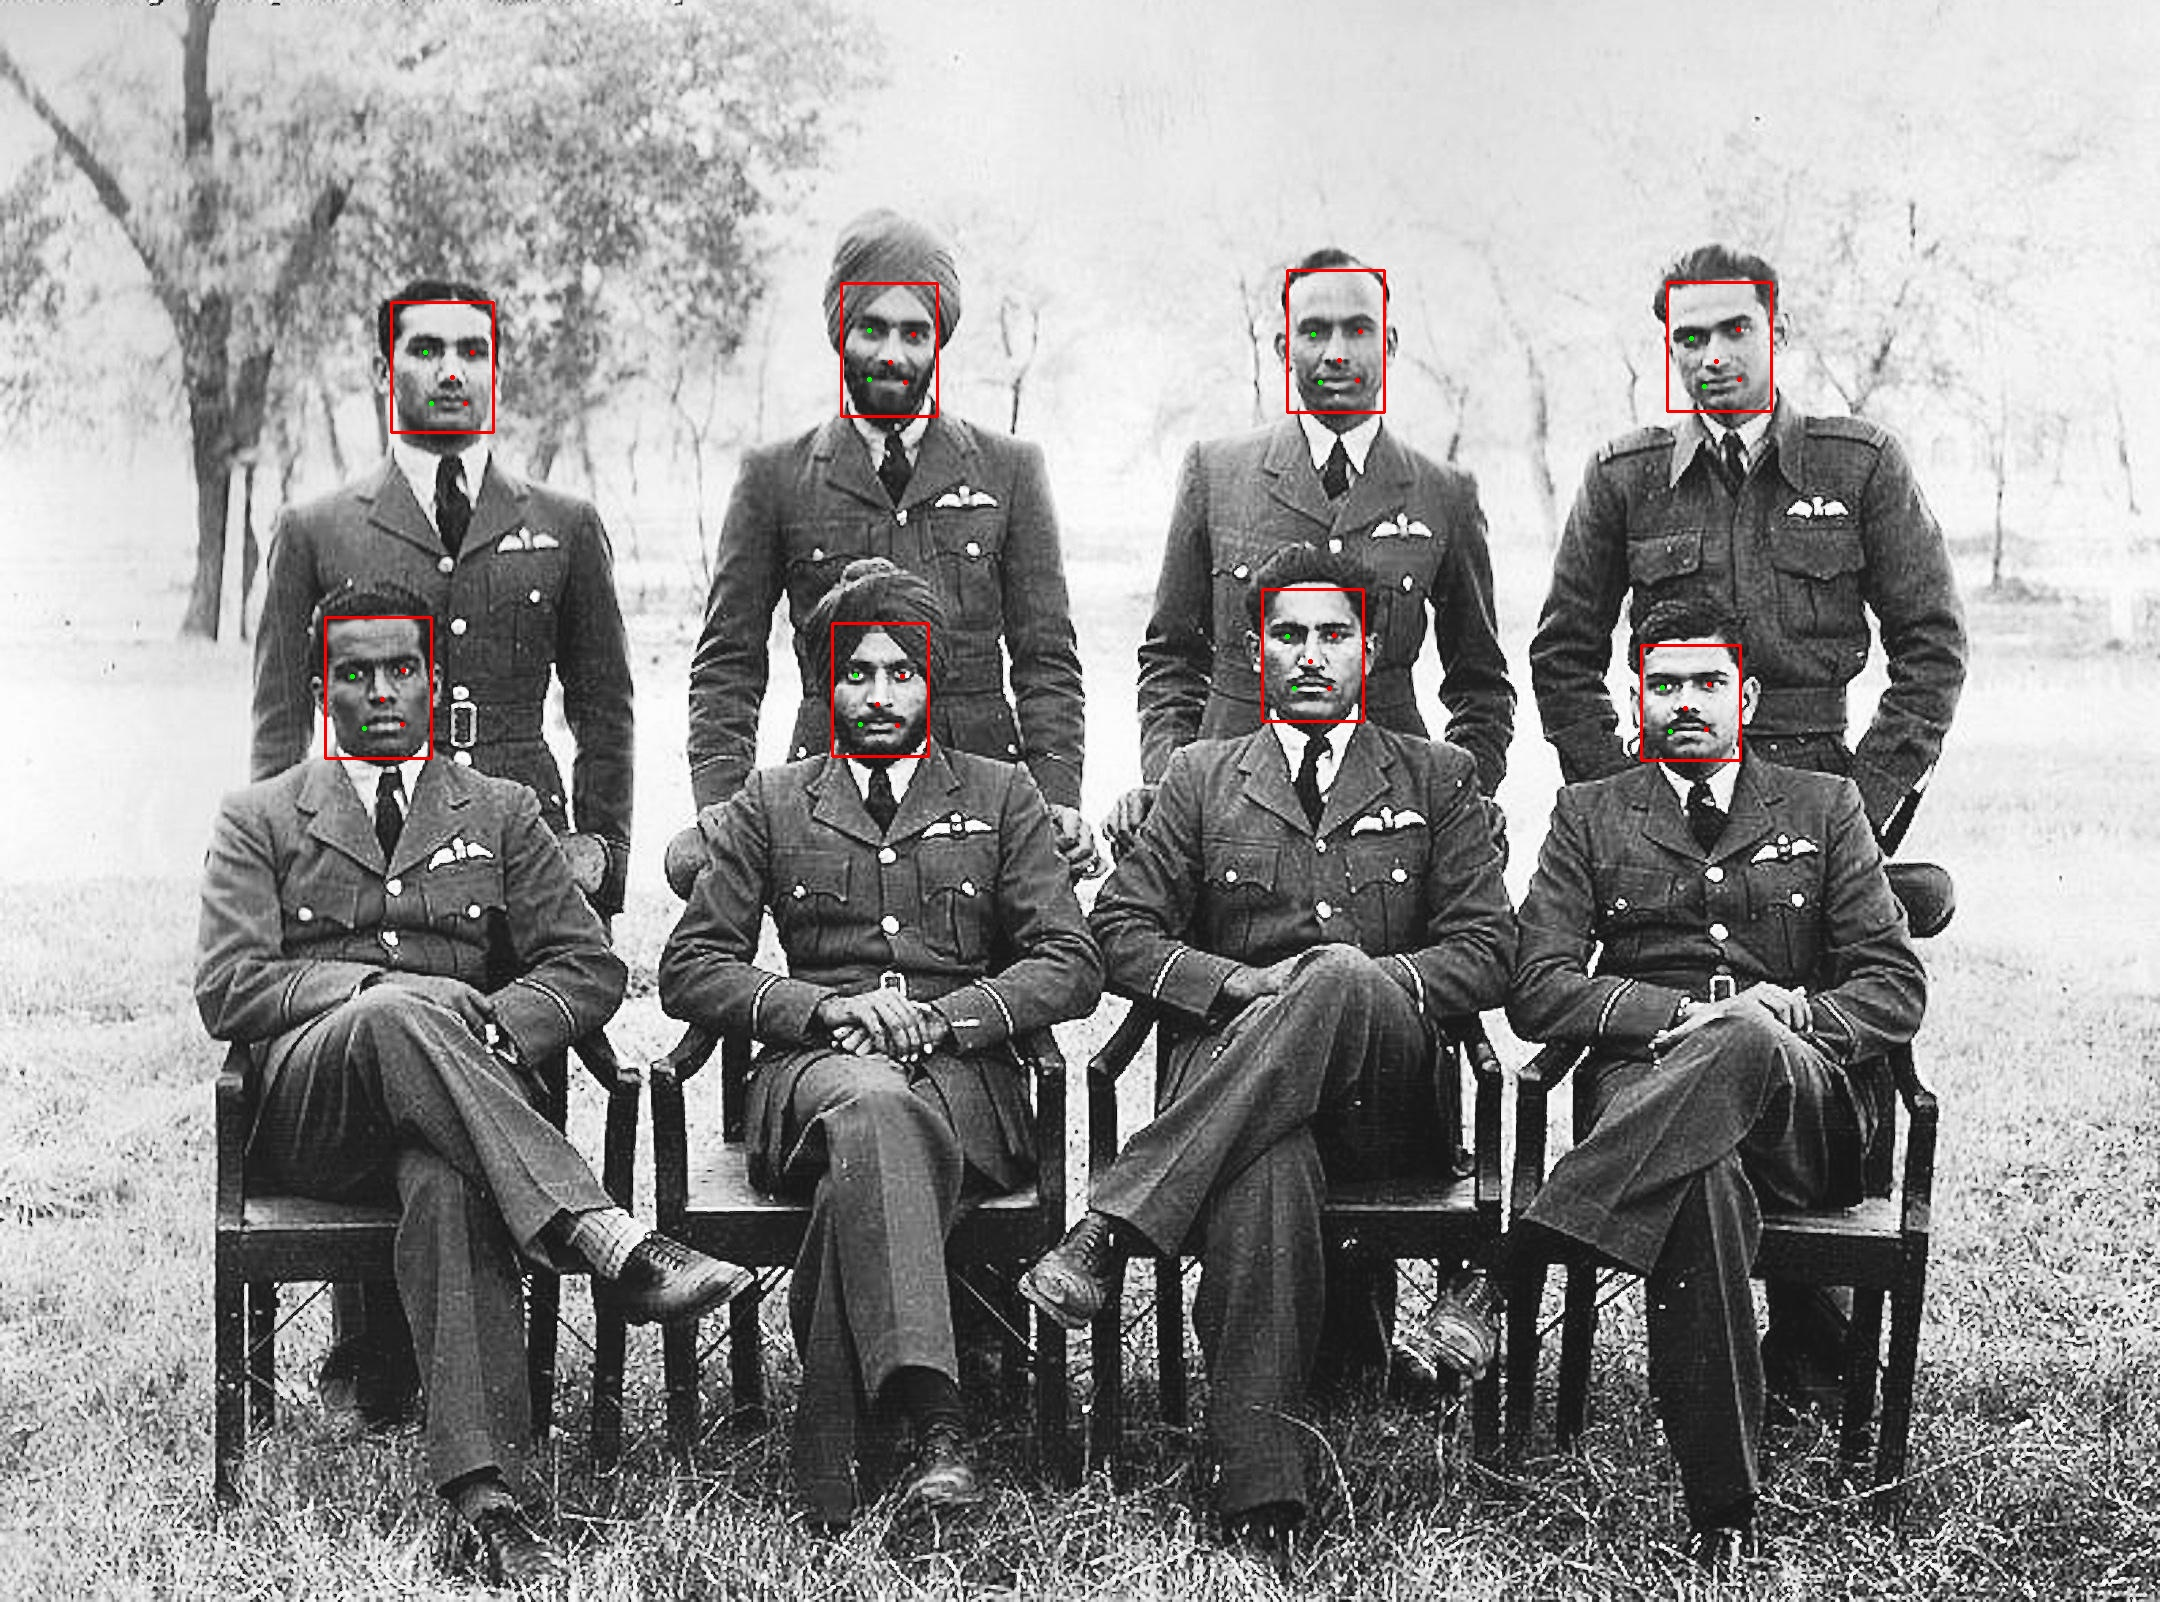
\includegraphics[width=\linewidth]{66.jpg}
	\caption{Output of test.py}
\end{figure}

To test \texttt{RetinaFace-50} on the original dataset created by us, we have modified the \texttt{test.py} file present in the original code. The original file took an image as input and produced an image with bounding boxes over faces as its output. We modified this file to produce the aforementioned image along with a .txt file with labels similar to that produced by the original program. All 105 images in the new dataset are run through this code and labels in form of text files are obtained for each of them. These labels are then compared to the true labels annotated in the creation of the dataset. 

\begin{wrapfigure}{r}{0.5\linewidth}
	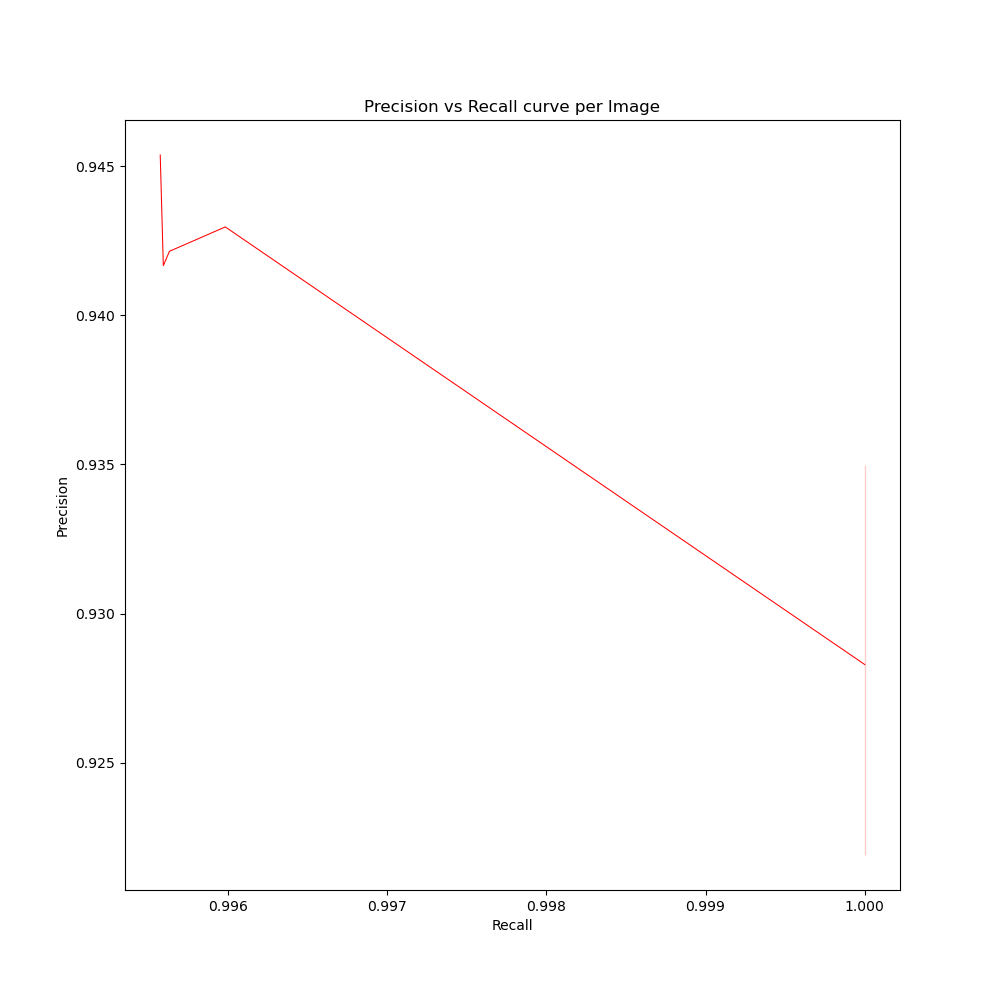
\includegraphics[width=\linewidth]{all.png}
	\caption{Precision Recall Curve for New Dataset}
\end{wrapfigure}

Instead of Box Voting, we have implemented an error margin method. If the bounding box created by the code is within $20$px of the box made manually, we mark this box as accurate. The precision and recall values for each image are noted and the resulting precision recall curve is shown below. The mean Average Precision for this dataset is $0.9197$.

The lack of smoothness of this curve is due to the small size of the new dataset. The dataset was not further broken down into difficulty or variation levels due to the same reason. Any further split would produce uninterpretable results. 

The code required to reproduce this along with the new dataset can be obtained at the github repository\footnote{\url{https://github.com/SohamSarfare/ADS}} created for the same.
\end{document}